\documentclass[12pt]{book}
\usepackage[a4paper, total={6in, 8in}]{geometry}
\usepackage{amssymb}
\usepackage{listings}
\usepackage{color}
\usepackage{graphicx}
\usepackage{subfig}
\usepackage{float}
\definecolor{mygrey}{gray}{.96} % Light Grey
\definecolor{BrickRed}{RGB}{120,0,0}


\def\xbf{\mathbf{x}}
\def\zbf{\mathbf{z}}
\def\xibf{\mathbf{\xi}}
\lstset{
	language=C++,              % choose the language of the code ("language=Verilog" is popular as well)
   tabsize=3,							  % sets the size of the tabs in spaces (1 Tab is replaced with 3 spaces)
	basicstyle=\footnotesize,               % the size of the fonts that are used for the code
	numbers=left,                   % where to put the line-numbers
	numberstyle=\footnotesize,              % the size of the fonts that are used for the line-numbers
	stepnumber=1,                   % the step between two line-numbers. If it's 1 each line will be numbered
	numbersep=5pt,                  % how far the line-numbers are from the code
	backgroundcolor=\color{mygrey}, % choose the background color. You must add \usepackage{color}
	showspaces=false,              % show spaces adding particular underscores
	showstringspaces=false,        % underline spaces within strings
	showtabs=false,                % show tabs within strings adding particular underscores
	frame=single,	                 % adds a frame around the code
	tabsize=3,	                    % sets default tabsize to 2 spaces
	captionpos=b,                   % sets the caption-position to bottom
	breaklines=true,                % sets automatic line breaking
	breakatwhitespace=false,        % sets if automatic breaks should only happen at whitespace
	%escapeinside={\%*}{*)},        % if you want to add a comment within your code
	commentstyle=\color{BrickRed}   % sets the comment style
}

\begin{document}
\title{\textbf{Monte Carlo Simulation Lab\\Assignment-5}}	
\author{Yash Vanjani\\(140123046)\\Mathematics and Computing\\IIT Guwahati}
\date{March 9th, 2016}

\maketitle

\newpage
\begin{enumerate}
\item[Q 1] Use the Box-Muller method and Marsaglia-Bray method to do the following :
(a) Generate a sample of 100, 500 and 10000 values from N (0, 1). Hence find the
sample mean and variance.\\
(b) Draw histogram in all cases.
\end{enumerate}
\noindent{Code of BOX-MULLER for R :}

\begin{lstlisting}
f<-function(x1,x2)
{
	return(sqrt(-2*log(x1))*cos(2*pi*x2))
}
g<-function(x1,x2)
{
	return(sqrt(-2*log(x1))*sin(2*pi*x2))
}
p<-c(100,500,10000)
z1<-vector("numeric")
z2<-vector("numeric")
for( i in 1:3)
{
	z1<-vector("numeric")
	z2<-vector("numeric")
	u1<-runif(p[i])
	u2<-runif(p[i])
	j<-1
	while(j<=p[i])
	{
		z1[j]=f(u1[j],u2[j])
		z2[j]=g(u1[j],u2[j])
		j=j+1
	}
	cat("Mean of ",p[i],"numbers of z1 is ",mean(z1),"\n")
	cat("Mean of ",p[i],"numbers of z2 is ",mean(z2),"\n")
	cat("Variance of ",p[i],"numbers of z1 is ",var(z1),"\n")
	cat("Variance of ",p[i],"numbers of z2 is ",var(z2),"\n")
	hist(z1,col="darkblue",main=paste("Normal Distribution(Z1) for n = ",p[i],"\nMean = ",mean(z1),"\nVariance = ",var(z1)),xlab="X",ylab="Frequency",breaks=p[i]/20)
	hist(z2,col="darkblue",main=paste("Normal Distribution(Z2) for n = ",p[i],"\nMean = ",mean(z2),"\nVariance = ",var(z2)),xlab="X",ylab="Frequency",breaks=p[i]/20)

}
\end{lstlisting}
\newpage
\underline{\textbf{Output :}}\\
\begin{lstlisting}
Mean of  100 numbers of z1 is  0.075\\ 
Mean of  100 numbers of z2 is  -0.073 \\
Variance of  100 numbers of z1 is  0.915\\ 
Variance of  100 numbers of z2 is  0.865 \\\\
Mean of  500 numbers of z1 is  -0.018 \\
Mean of  500 numbers of z2 is  -0.001 \\
Variance of  500 numbers of z1 is  1.039\\ 
Variance of  500 numbers of z2 is  0.924 \\\\
Mean of  10000 numbers of z1 is  -0.002 \\
Mean of  10000 numbers of z2 is  0.005 \\
Variance of  10000 numbers of z1 is  1.003\\ 
Variance of  10000 numbers of z2 is  0.999 \\\\
\end{lstlisting}
\newpage
The histograms are shown below:
\begin{figure}[H]
	\centering
	\subfloat{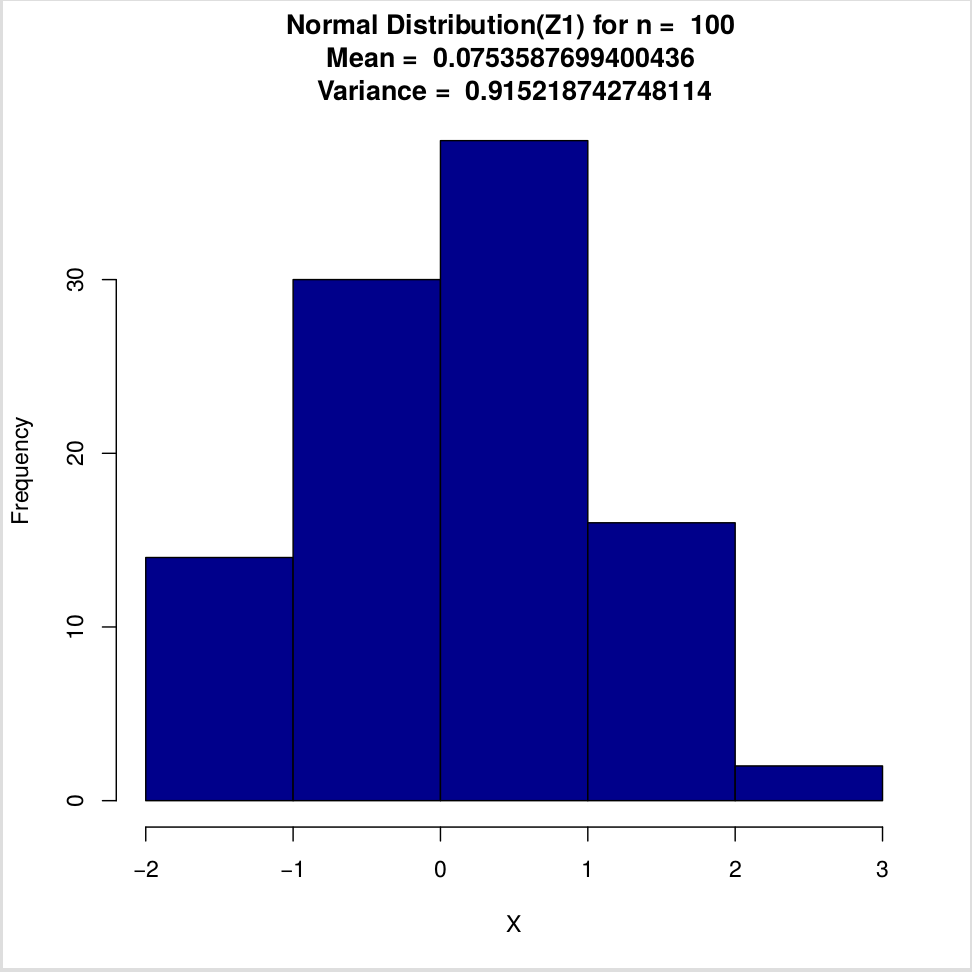
\includegraphics[width=0.6\textwidth]{1_1_1.png}}	
\end{figure}
\begin{figure}[H]
	\centering
	\subfloat{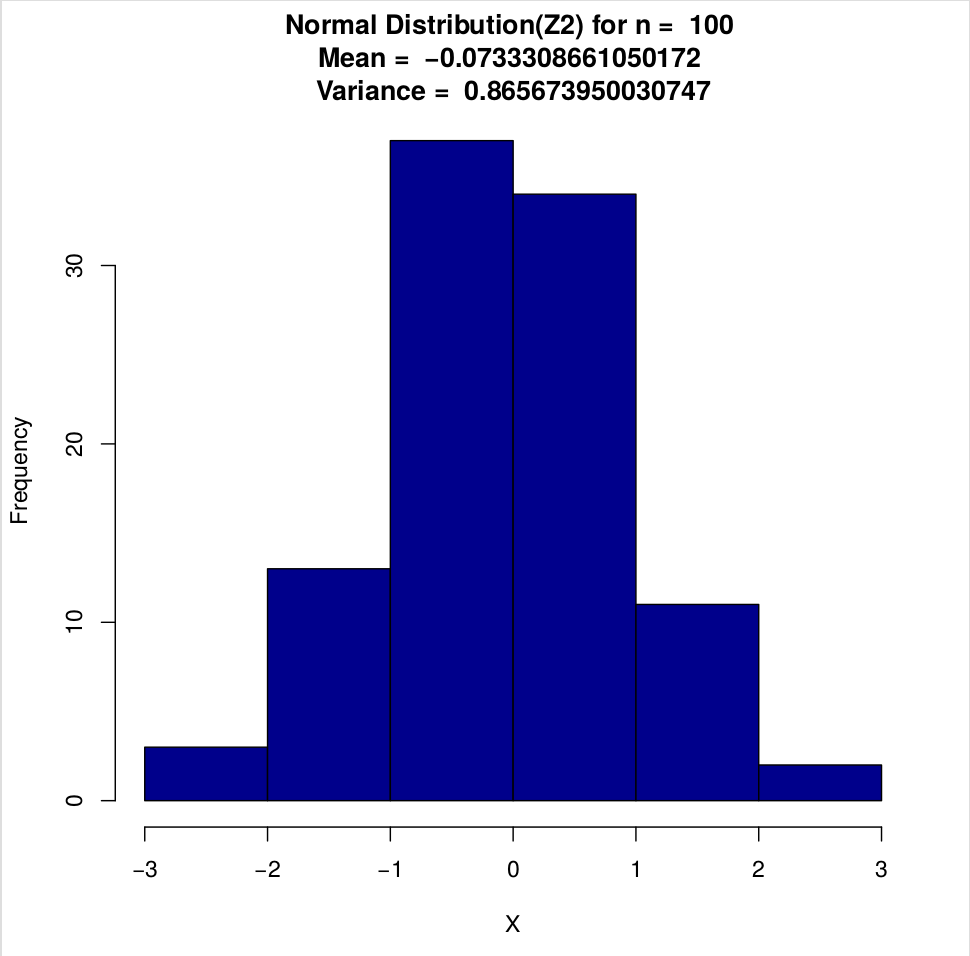
\includegraphics[width=0.6\textwidth]{1_1_2.png}}	
\end{figure}
\begin{figure}[H]
	\centering
	\subfloat{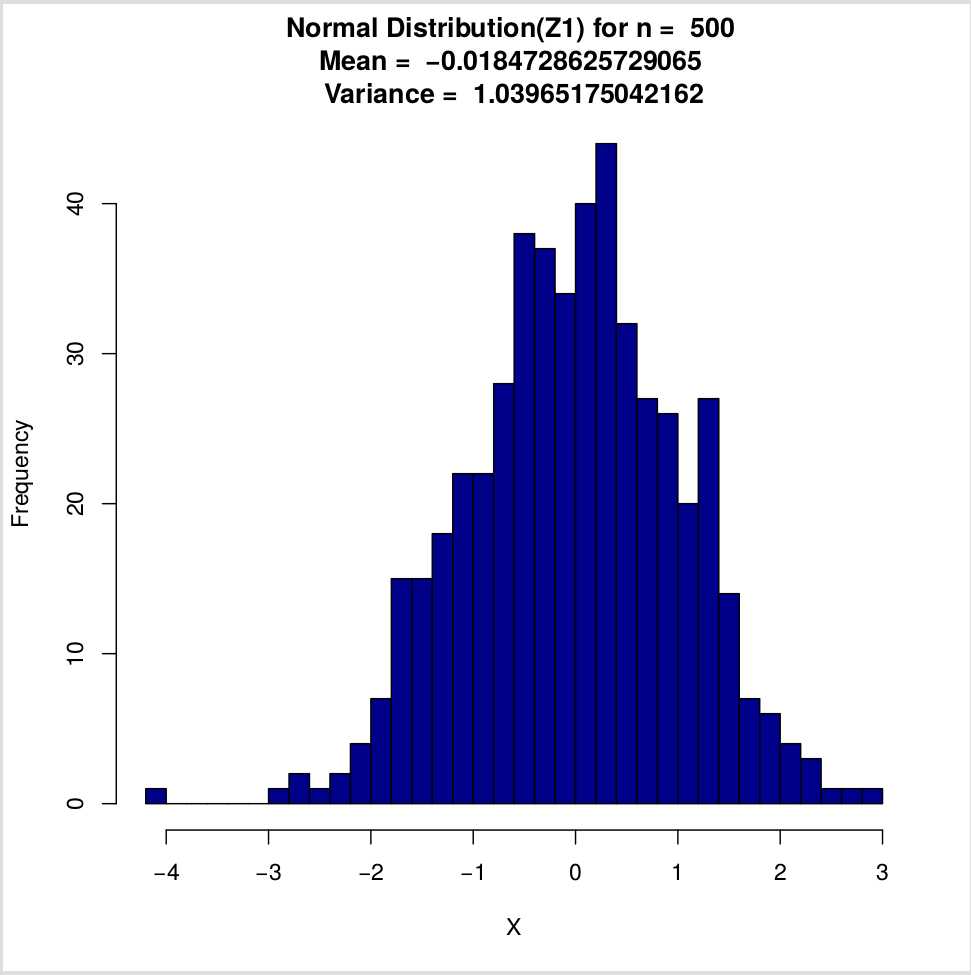
\includegraphics[width=0.6\textwidth]{1_1_3.png}}	
\end{figure}
\begin{figure}[H]
	\centering
	\subfloat{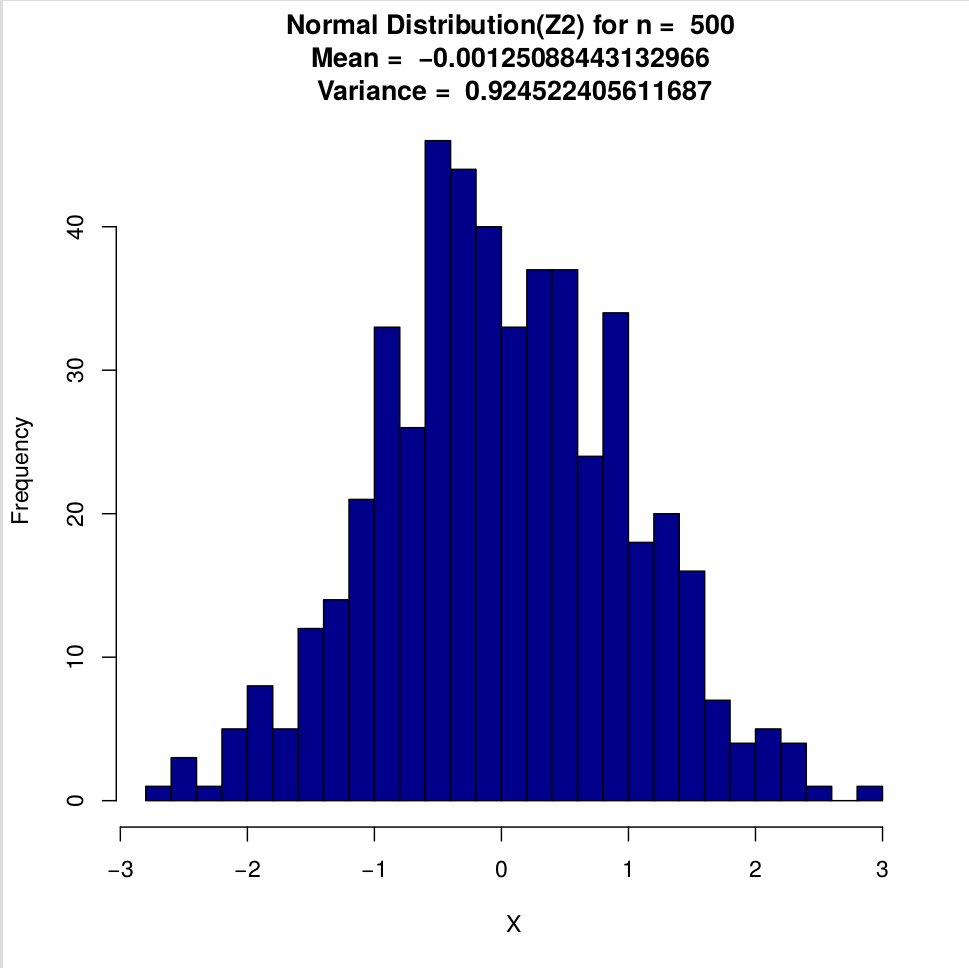
\includegraphics[width=0.6\textwidth]{1_1_4.png}}	
\end{figure}
\begin{figure}[H]
	\centering
	\subfloat{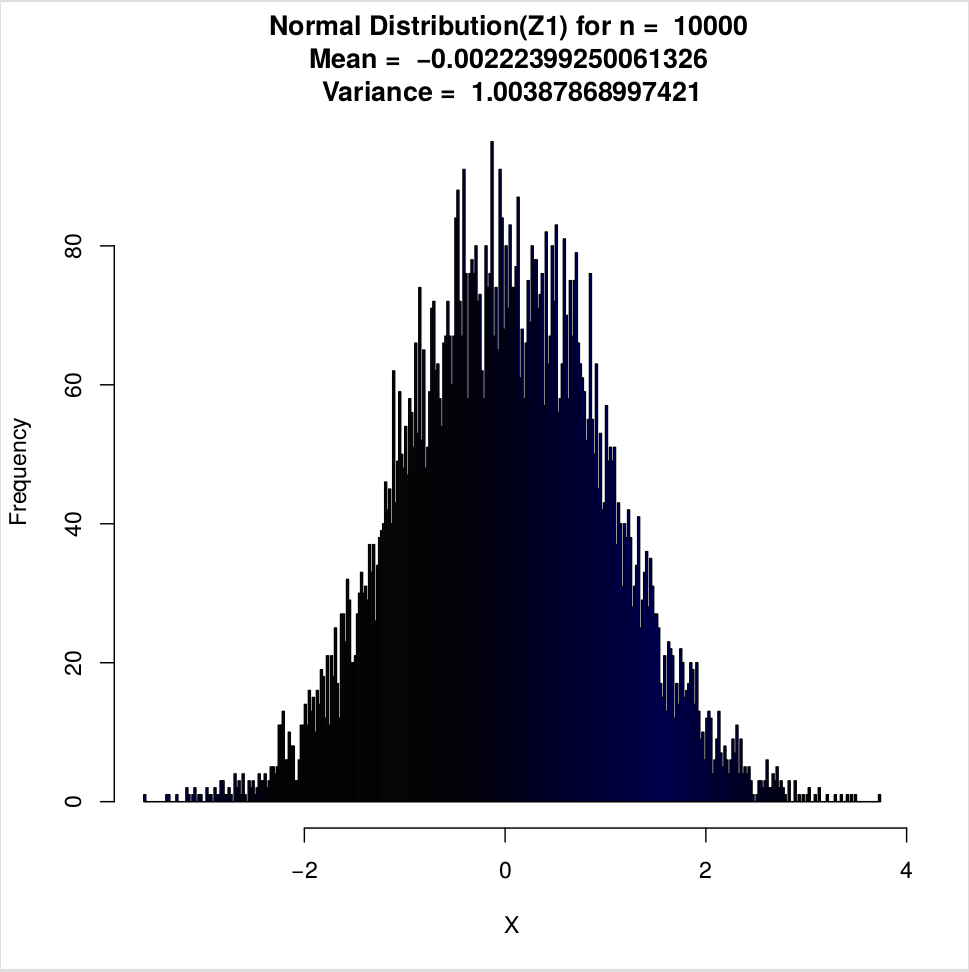
\includegraphics[width=0.6\textwidth]{1_1_5.png}}	
\end{figure}
\begin{figure}[H]
	\centering
	\subfloat{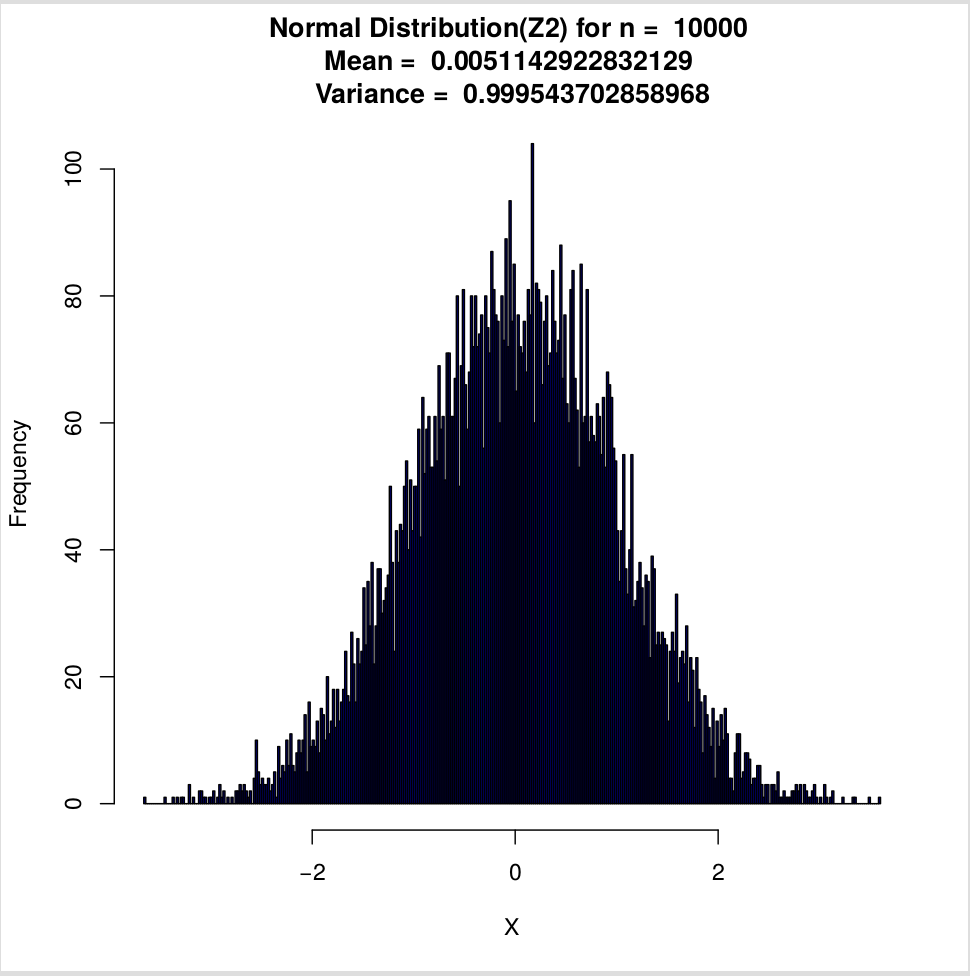
\includegraphics[width=0.6\textwidth]{1_1_6.png}}	
\end{figure}
\newpage
The code for MARSAGLIA-BRAY for R:\\
\begin{lstlisting}
f<-function(v1,v2)
{
	return(v1*sqrt(-2*log(v1^2+v2^2)/(v1^2+v2^2)))
}
g<-function(v1,v2)
{
	return(v2*sqrt(-2*log(v1^2+v2^2)/(v1^2+v2^2)))
}
p<-c(100,500,10000)
for(i in 1:3)
{
	v1<-2*runif(p[i])-1
	v2<-2*runif(p[i])-1
	j<-1
	k<-1
	z1<-vector("numeric")
	z2<-vector("numeric")
	while(j<=p[i])
	{
		if(v1[j]^2+v2[j]^2<1)
		{
			z1[k]<-f(v1[j],v2[j])
			z2[k]<-g(v1[j],v2[j])
			k=k+1
		}
		j=j+1
	}
	cat("Mean of ",p[i],"numbers of z1 is ",mean(z1),"\n")
	cat("Mean of ",p[i],"numbers of z2 is ",mean(z2),"\n")
	cat("Variance of ",p[i],"numbers of z1 is ",var(z1),"\n")
	cat("Variance of ",p[i],"numbers of z2 is ",var(z2),"\n")
	hist(z1,col="darkblue",main=paste("Normal Distribution(Z1) for n = ",p[i],"\nMean = ",mean(z1),"\nVariance = ",var(z1)),xlab="X",ylab="Frequency",breaks=p[i]/20)
	hist(z2,col="darkblue",main=paste("Normal Distribution(Z2) for n = ",p[i],"\nMean = ",mean(z2),"\nVariance = ",var(z2)),xlab="X",ylab="Frequency",breaks=p[i]/20)
}
\end{lstlisting}
\newpage
\underline{\textbf{Output :}}\\
\begin{lstlisting}
Mean of  100 numbers of z1 is  -0.146\\ 
Mean of  100 numbers of z2 is  0.014 \\
Variance of  100 numbers of z1 is  0.847\\ 
Variance of  100 numbers of z2 is  0.986 \\\\
Mean of  500 numbers of z1 is  0.087 \\
Mean of  500 numbers of z2 is  0.012 \\
Variance of  500 numbers of z1 is  1.094\\ 
Variance of  500 numbers of z2 is  0.054 \\\\
Mean of  10000 numbers of z1 is  0.012 \\
Mean of  10000 numbers of z2 is  0.004 \\
Variance of  10000 numbers of z1 is  0.984\\ 
Variance of  10000 numbers of z2 is  1.040\\\\
\end{lstlisting}
\newpage
The histograms are shown below:
\begin{figure}[H]
	\centering
	\subfloat{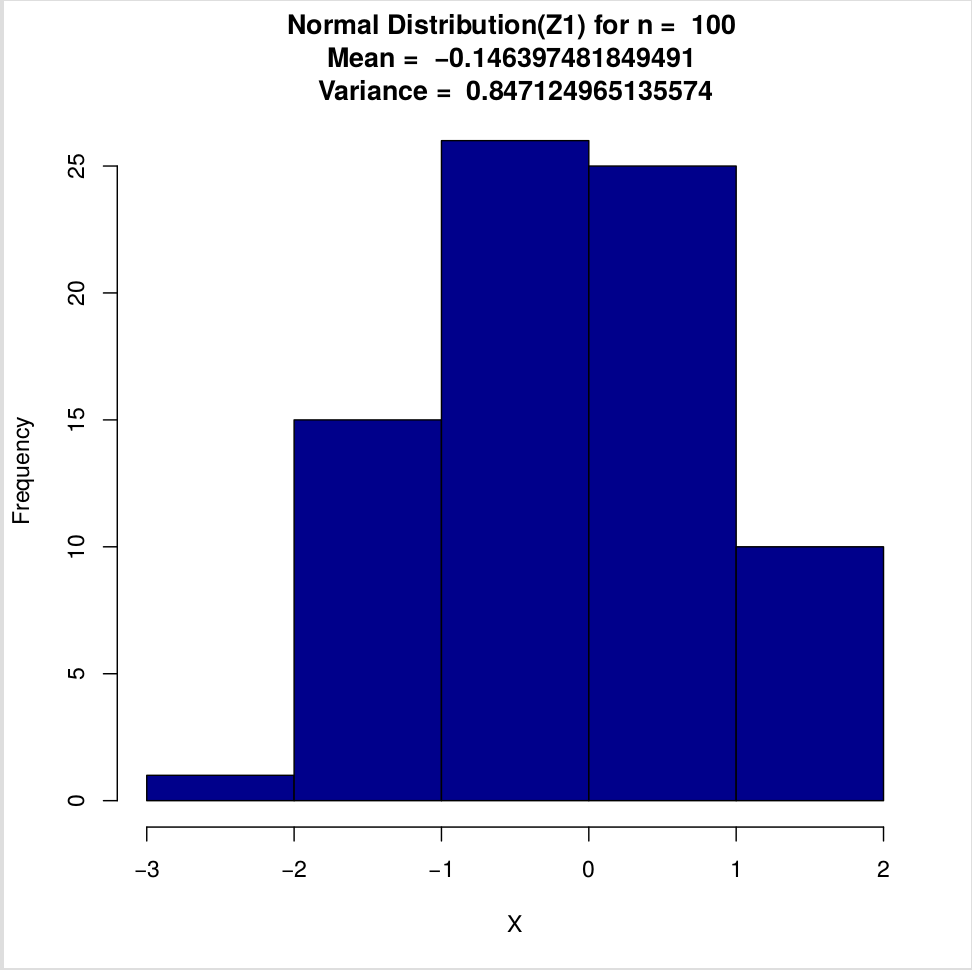
\includegraphics[width=0.6\textwidth]{1_2_1.png}}	
\end{figure}
\begin{figure}[H]
	\centering
	\subfloat{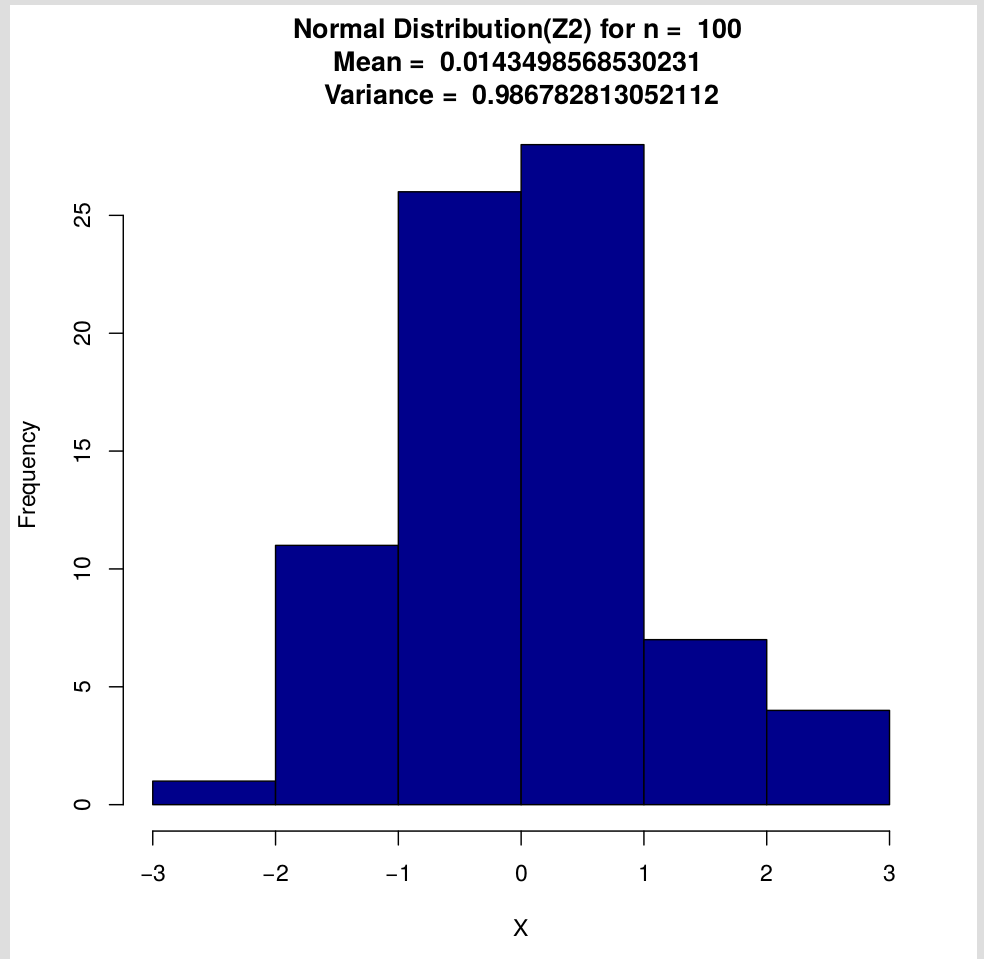
\includegraphics[width=0.6\textwidth]{1_2_2.png}}	
\end{figure}
\begin{figure}[H]
	\centering
	\subfloat{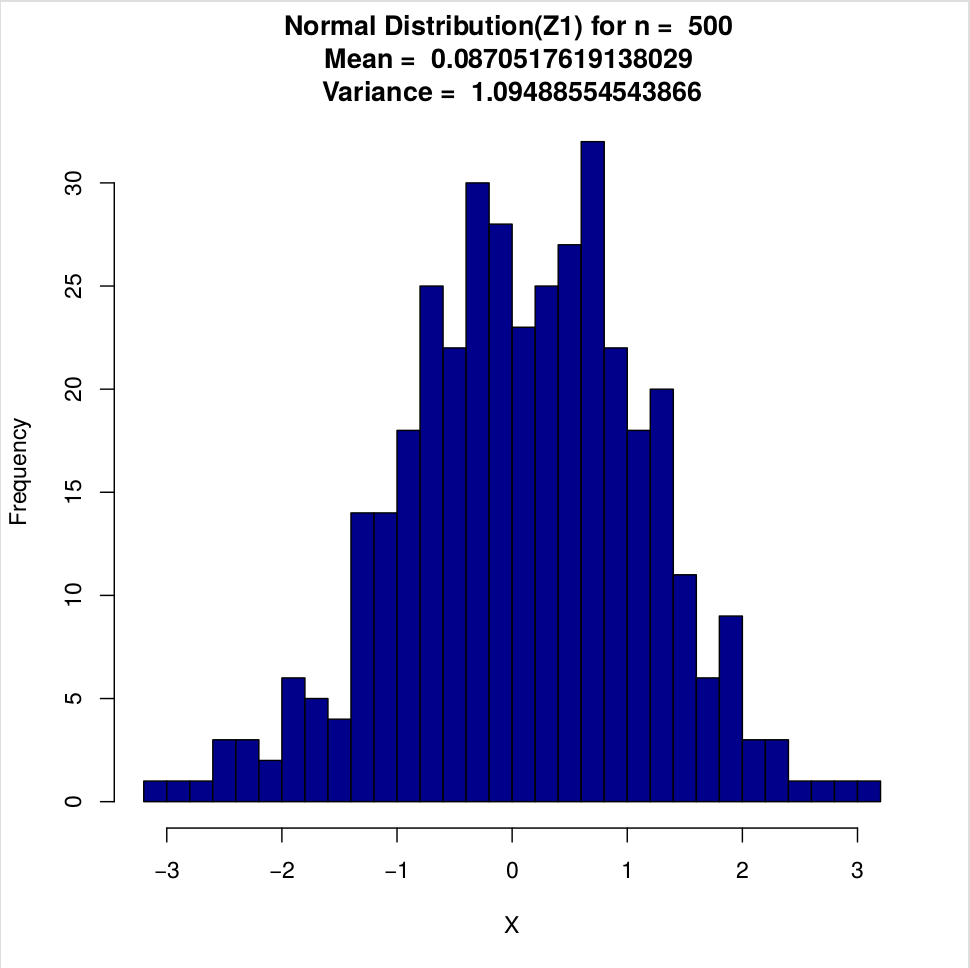
\includegraphics[width=0.6\textwidth]{1_2_3.png}}	
\end{figure}
\begin{figure}[H]
	\centering
	\subfloat{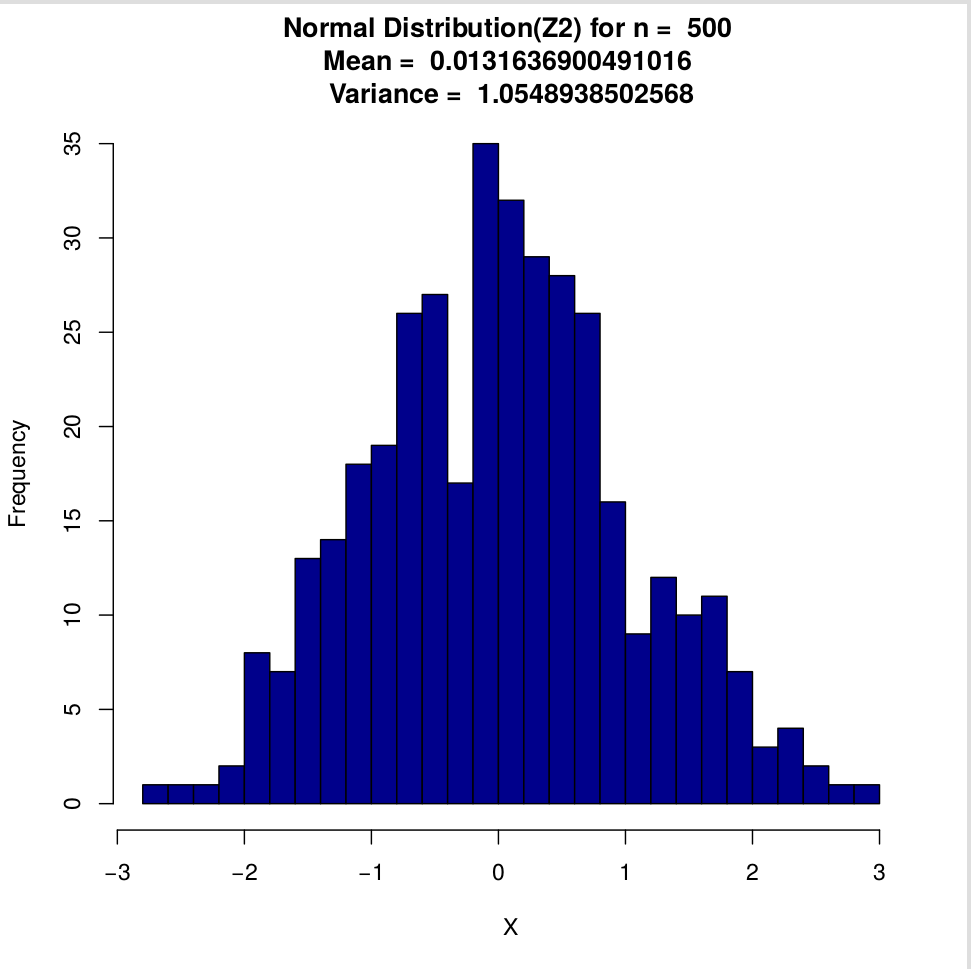
\includegraphics[width=0.6\textwidth]{1_2_4.png}}	
\end{figure}
\begin{figure}[H]
	\centering
	\subfloat{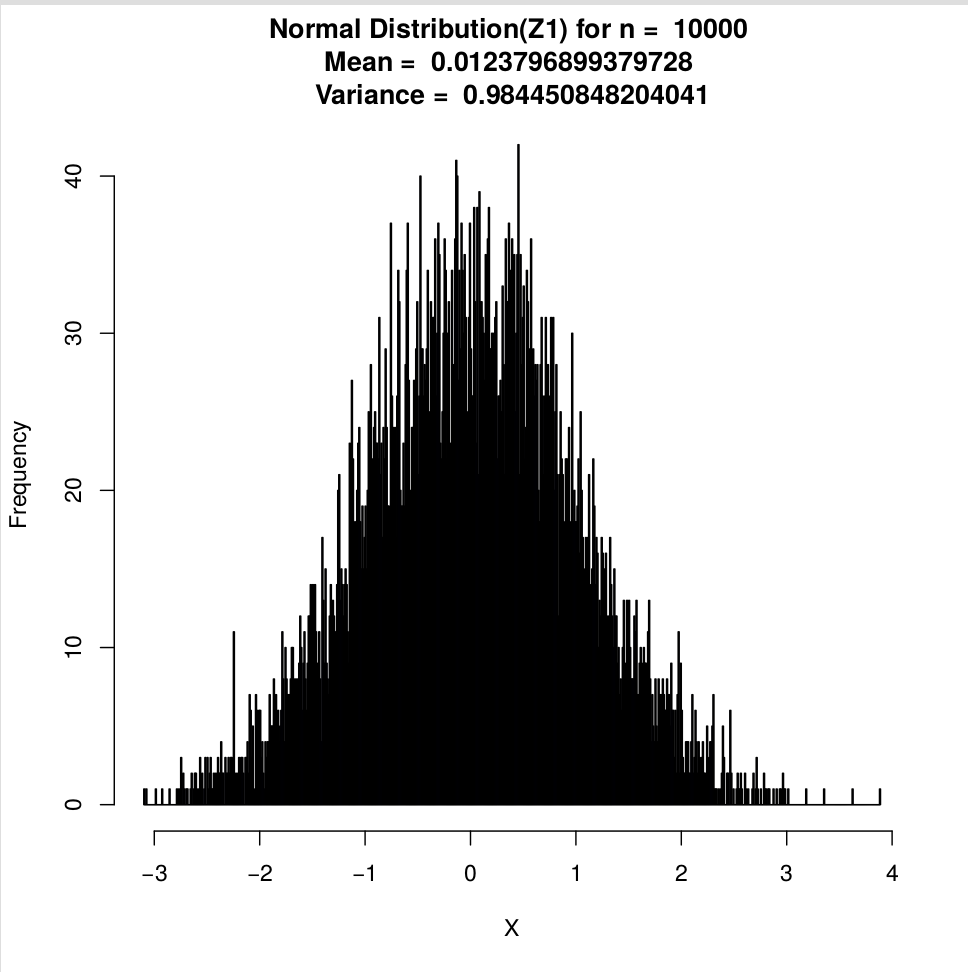
\includegraphics[width=0.6\textwidth]{1_2_5.png}}	
\end{figure}
\begin{figure}[H]
	\centering
	\subfloat{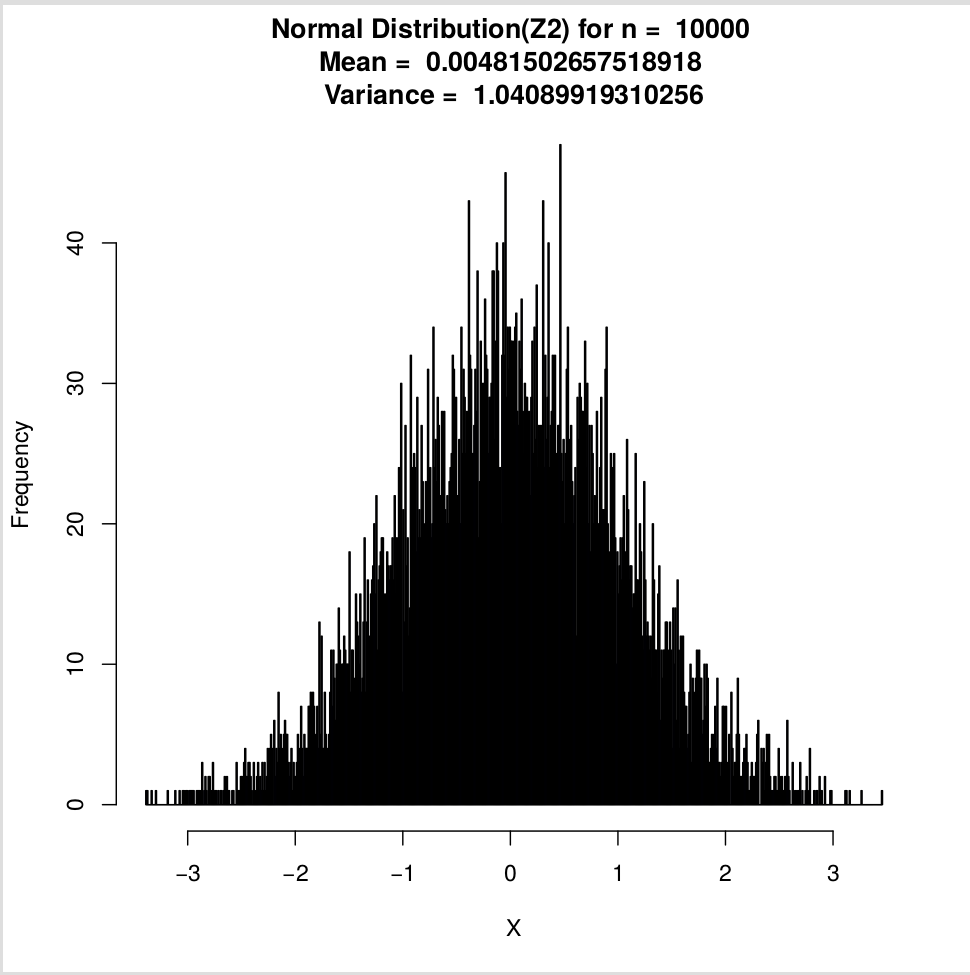
\includegraphics[width=0.6\textwidth]{1_2_6.png}}	
\end{figure}
\newpage
\noindent{\textbf{\underline{Observations :}}}

\begin{enumerate}
\item The mean of the distribution calculated using both the methods comes out to be nearly equal to 0 which is in fact the mean of Standard Normal Distribution.
\item The variance of these values indicate that they are going towards 1 which is equal to the theoretical value of the variance and thus the given Random variable actually has a distribution which is the same as the Normal Distribution with variance 1 and mean 0. Furthermore the histograms resemble those of Normal Distribution.
\item There are two methods which can be used to generate the Normal Distribution: Box-Muller and Marsaglia-Bray, both of them as shown above give nearly same precision but in the first one all the random numbers generated are used while in the other method the random numbers generated are checked whether that they are inside the circle of radius 1 before proceding further.
\item When the number of sample random variables is taken to as large as 10,000, the normal distribution of Random variables becomes visible.
\item The probability density graph is symmetric about mean.
\end{enumerate}
\newpage
\begin{enumerate}
\item[Q 2] Now use the above generated values to generated samples from $N(\mu = 0;\sigma^2 = 5)$ and $N(\mu = 5;\sigma^2 = 5)$. Hence plot the empirical(from sample with size 500) distribution function and theoretical distribution function in the same plot.
\end{enumerate}
\noindent{Code for R: }

\begin{lstlisting}
f<-function(x1,x2)
{
	return(sqrt(-2*log(x1))*cos(2*pi*x2))
}
g<-function(x1,x2)
{
	return(sqrt(-2*log(x1))*sin(2*pi*x2))
}
p<-c(100,500,1000)
z1<-vector("numeric")
z2<-vector("numeric")
for( i in 1:3)
{
	z1<-vector("numeric")
	z2<-vector("numeric")
	u1<-runif(p[i])
	u2<-runif(p[i])
	j<-1
	while(j<=p[i])
	{
		z1[j]=sqrt(5)*f(u1[j],u2[j])
		z2[j]=(sqrt(5)*g(u1[j],u2[j]))+5
		j=j+1
	}
	cat("Mean of ",p[i],"numbers of z1 is ",mean(z1),"\n")
	cat("Mean of ",p[i],"numbers of z2 is ",mean(z2),"\n")
	cat("Variance of ",p[i],"numbers of z1 is ",var(z1),"\n")
	cat("Variance of ",p[i],"numbers of z2 is ",var(z2),"\n")
	#hist(z1,col="darkblue",main=paste("Normal Distribution(Z1) for n = ",p[i],"\nMean = ",mean(z1),"\nVariance = ",var(z1)),xlab="X",ylab="Frequency",breaks=p[i]/20)
	#hist(z2,col="darkblue",main=paste("Normal Distribution(Z2) for n = ",p[i],"\nMean = ",mean(z2),"\nVariance = ",var(z2)),xlab="X",ylab="Frequency",breaks=p[i]/20)

	if(p[i]==500)
	{
		xseq<-seq(-10,15,0.01);
		h=ecdf(z1)
		m=ecdf(z2)
	    cumulative<-pnorm(xseq,0,sqrt(5))
	    plot(xseq, cumulative, col="darkorange", xlab="", ylab="Cumulative Probability",type="l",lwd=2, cex=2, main="CDF of Mean = 0\n Variance = 5", cex.axis=.8) 
	lines(h,col="blue")

	cum<-pnorm(xseq,5,sqrt(5))
	plot(xseq, cum, col="darkorange", xlab="", ylab="Cumulative Probability",type="l",lwd=2, cex=2, main="CDF of Mean = 5\n Variance = 5", cex.axis=.8)
	lines(m,col="darkgreen") 
	}
}
\end{lstlisting}
Plots of the emperical distribution function and theoritical distribution function is as follows:\\\\
\begin{figure}[H]
	\centering
	\subfloat{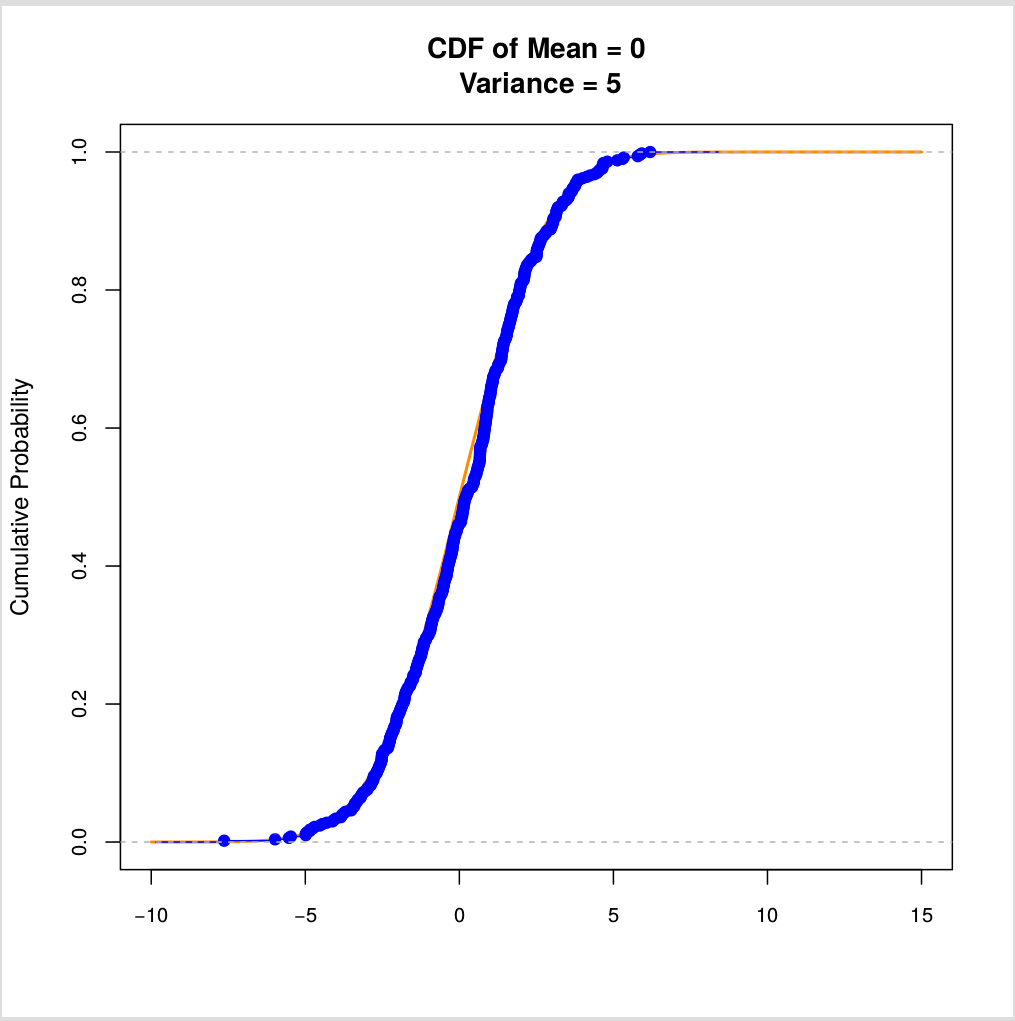
\includegraphics[width=0.6\textwidth]{2_1.png}}	
\end{figure}
\begin{figure}[H]
	\centering
	\subfloat{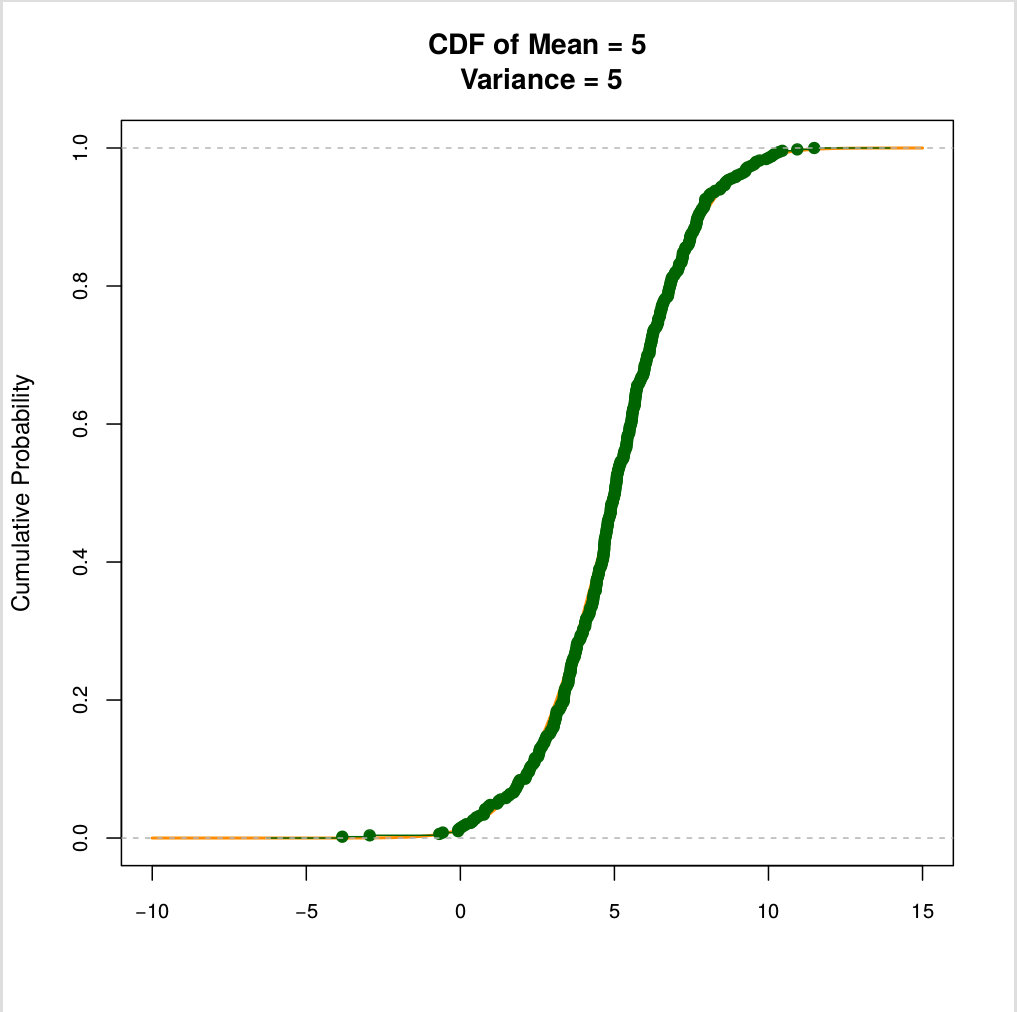
\includegraphics[width=0.6\textwidth]{2_2.png}}	
\end{figure}
\newpage
\begin{enumerate}
\item[Q 3] Keep a track of the computational time required for both the methods. Which method is faster ?
\end{enumerate}
\noindent{Code of R for BOX-MULLER method :}\\
\begin{lstlisting}
f<-function(x1,x2)
{
	return(sqrt(-2*log(x1))*cos(2*pi*x2))
}
g<-function(x1,x2)
{
	return(sqrt(-2*log(x1))*sin(2*pi*x2))
}
p<-c(10^3,10^4,10^5)
z1<-vector("numeric")
z2<-vector("numeric")
for( i in 1:3)
{
	ptm<-proc.time()
	z1<-vector("numeric")
	z2<-vector("numeric")
	u1<-runif(p[i])
	u2<-runif(p[i])
	j<-1
	while(j<=p[i])
	{
		z1[j]=f(u1[j],u2[j])
		z2[j]=g(u1[j],u2[j])
		j=j+1
	}
	cat("\n For n = ",p[i],"The time taken by Box muller method\n")
	print(proc.time() - ptm)

}
\end{lstlisting}
\noindent{\textbf{\underline{\textbf{Output :}}}}\\
\begin{table}[h!]
\centering
\begin{tabular}{||c|c|c| c|c||}
\hline
&USER &SYSTEM&ELAPSED \\
[0.5ex]
\hline\hline
n=100&0.0110&0.000&0.011\\	
n=500&0.254&0.000&0.253\\
n=10000&31.498&2.757&34.241\\
[1ex]
\hline
\end{tabular}
\caption{Time taken by BOX-MULLER method}
\label{table:1}
\end{table}\\
\newpage
\noindent{Code of R for MARSAGLIA-GRAY method :}\\
\begin{lstlisting}
f<-function(v1,v2)
{
	return(v1*sqrt(-2*log(v1^2+v2^2)/(v1^2+v2^2)))
}
g<-function(v1,v2)
{
	return(v2*sqrt(-2*log(v1^2+v2^2)/(v1^2+v2^2)))
}
p<-c(100,500,10000)
for(i in 1:3)
{
	ptm<-proc.time()
	v1<-2*runif(p[i])-1
	v2<-2*runif(p[i])-1
	j<-1
	k<-1
	z1<-vector("numeric")
	z2<-vector("numeric")
	while(j<=p[i])
	{
		if(v1[j]^2+v2[j]^2<1)
		{
			z1[k]<-f(v1[j],v2[j])
			z2[k]<-g(v1[j],v2[j])
			k=k+1
		}
		j=j+1
	}
	cat("\n For n = ",p[i]," The time taken by Marsaglia Bray method\n")
	print(proc.time() - ptm)
}
\end{lstlisting}


\noindent{\textbf{\underline{\textbf{Output :}}}}\\
\begin{table}[h!]
\centering
\begin{tabular}{||c|c|c| c|c||}
\hline
&USER &SYSTEM&ELAPSED \\
[0.5ex]
\hline\hline
n=100&0.001&0.000&0.001\\	
n=500&0.005&0.001&0.006\\
n=10000&0.198&0.007&0.206\\
[1ex]
\hline
\end{tabular}
\caption{Time taken by MARSAGLIA-BRAY method method}
\label{table:1}
\end{table}\\
\newpage
\noindent{\textbf{\underline{Observation : }}}\\

\begin{enumerate}
\item As expected we observe that MARSAGLIA-BRAY method takes very very less time than BOX-MULLER method to compute random numbers.
\item MARSAGLIA-BRAY method is almost 150x faster than BOX-MULLER method.

\end{enumerate}

\newpage
\begin{enumerate}
\item[Q 4] For the Marsaglia-Bray method keep track of the proportional of values rejected. How does it compare with $1 - \frac{\pi}{4} ?$
\end{enumerate}
\noindent{Code of R for MARSAGLIA-GRAY method : }\\
\begin{lstlisting}
f<-function(v1,v2)
{
	return(v1*sqrt(-2*log(v1^2+v2^2)/(v1^2+v2^2)))
}
g<-function(v1,v2)
{
	return(v2*sqrt(-2*log(v1^2+v2^2)/(v1^2+v2^2)))
}
p<-c(100,500,10000)
for(i in 1:3)
{
	accepted<-array(0,p[i])
	v1<-2*runif(p[i])-1
	v2<-2*runif(p[i])-1
	j<-1
	k<-1
	z1<-vector("numeric")
	z2<-vector("numeric")
	while(j<=p[i])
	{
		if(v1[j]^2+v2[j]^2<1)
		{
			z1[k]<-f(v1[j],v2[j])
			z2[k]<-g(v1[j],v2[j])
			k=k+1
			accepted[j]=accepted[j]+1

		}
		j=j+1
	}
	cat("Number of values accepted for ",p[i],"numbers is ",sum(accepted),"\n")
	cat("Rejection probability =  ",1-(sum(accepted)/p[i]),"\n")

}
\end{lstlisting}
\newpage
\noindent{\textbf{\underline{\textbf{Output :}}}}\\
\begin{table}[h!]
\centering
\begin{tabular}{||c|c||}
\hline
&Rejection Probability \\
[0.5ex]
\hline\hline
n=100&0.16\\	
n=500&0.216\\
n=10000&0.2187\\
[1ex]
\hline
\end{tabular}
\caption{Rejection Probabaility}
\label{table:1}
\end{table}\\

\end{document}